% !TeX spellcheck = de_DE
\section{Strategien zur Parallelisierung}
Es gibt mehrere Möglichkeiten zur Umsetzung einer Parallelisierung, sowie verschiedene Schwerpunkte, welche diese haben kann. Die Analyse der sequenziellen Implementierung hat gezeigt, dass die \emph{Evaluation Time} den größten Einfluss auf die Ausführungszeit hat.  Dementsprechend kann bei einer erfolgreichen Parallelisierung dieser Phase die größte Reduktion der Ausführungszeit erzielt werden. Aus diesem Grund liegt der Fokus im Weiteren hierauf. 
\begin{figure}[!h]
	\centering
	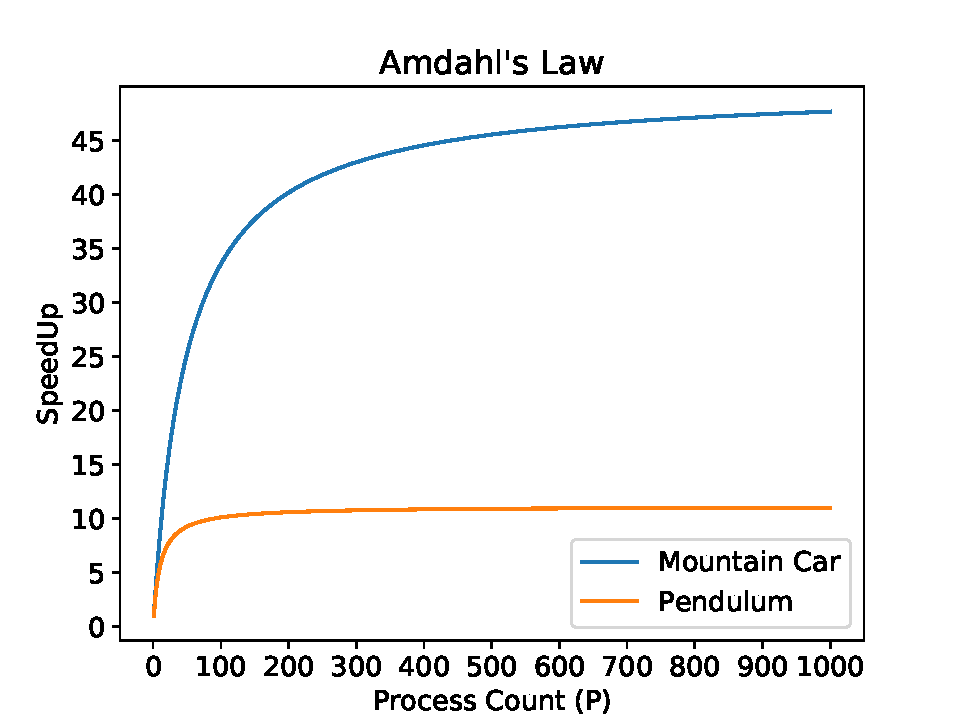
\includegraphics[width=0.5\textwidth]{./img/ahmdals_law_mountain_pendulum.pdf} 
	\caption{Durch \emph{Amdahl's Law} berechnete theoretische \emph{SpeedUp} für das \emph{Mountain Car} und \emph{Pendulum} Problem in Abhängigkeit der Anzahl an Prozessen}
	\label{fig:amdahls_law_mountain_pendulum}
\end{figure}
Mit \emph{Amdahl's Law}, welches in Kapitel \ref{subsec:basics_performance} vorgestellt ist, kann der theoretisch erreichbare \emph{SpeedUp} in Abhängigkeit von $P$ Prozessoren berechnet werden. Dies ist in Abbildung \ref{fig:amdahls_law_mountain_pendulum} dargestellt, wobei entsprechend der Analyseergebnisse angenommen wird, dass die \emph{Mountain Car} Umgebung zu $98\%$ und die \emph{Pendulum} Umgebung zu $91\%$ parallelisiert werden können. Durch die Abbildung ist ersichtlich, dass beide Probleme anfänglich mit steigender Anzahl an Prozessen sehr gute \emph{SpeedUp} Werte erzielen. Allerdings ist das Hinzufügen von weiterer Rechenleistung ab einem gewissen Punkt nicht mehr effektiv, da der Anstieg des \emph{SpeedUps} zunehmend geringer wird und schlussendlich gegen einen gewissen Wert konvergiert. Für $P \rightarrow \infty$ liegt der maximale \emph{SpeedUp} für die \emph{Mountain Car} Umgebung bei Faktor 50 und für die \emph{Pendulum} Umgebung bei Faktor $11.\overline{1}$. Auch wenn diese Ergebnisse eine ungefähre Richtlinie bieten, ist das Erreichen dieser Vorgaben in einer praktischen Umsetzung unwahrscheinlich. Durch eine hohe Anzahl an beteiligten Prozessen entsteht in der Regel ein hoher Kommunikationsaufwand, der sich negativ auf den \emph{SpeedUp} Wert auswirkt. Im Folgenden werden verschiedene Strategien zur Umsetzung einer möglichst effizienten Parallelisierung aufgezeigt und die verschiedenen Vor- und Nachteile dieser gegeneinander abgewogen.
\\\\
Vor dem Auswählen einer geeigneten Strategie sollen die zu parallelisierenden Funktionen der \emph{Evaluation Time} analysiert werden. Im sequenziellen Verfahren wird in dieser Phase über eine Liste mit allen Agenten iteriert. Für jeden von diesen wird die Umgebung einmal zurückgesetzt und ein \ac{KNN} aus dem Genom des Agenten gebildet. Danach wird die Umgebung simuliert. Bei diesem Vorgang können beliebig viele Simulationsschritte und Aktivierungen des \ac{KNN} ausgeführt werden. 
\\\\
Ein möglicher Ansatz besteht darin, die Berechnungen in einem \ac{KNN} selbst zu parallelisieren. Dies ist eine valide Strategie, die unter anderem von Bibliotheken wie Tensorflow und Pytorch genutzt wird. Die einzelnen Neuronen einer Schicht können beispielsweise unabhängig voneinander aktiviert und somit auch parallelisiert werden. Zusätzlich kann eine solche Parallelisierung nicht nur mithilfe von \acp{CPU}, sondern auch auf \acp{GPU} umgesetzt werden. Diese haben in der Regel mehr unabhängige Prozessoren als normale \acp{CPU}, wodurch in vielen Fällen eine bessere Parallelisierung ermöglicht wird. Allerdings sprechen zwei Gründe gegen den Einsatz einer solchen Parallelisierungsstrategie in dieser Arbeit. Die vorgestellten Bibliotheken implementieren diese Funktionalitäten bereits, sind weit verbreitet und für verschiedene Plattformen optimiert. Zusätzlich ist es im Rahmen einer zukünftigen Erweiterung möglich, diese einfach in dieses Projekt zu integrieren. Daher ist es nicht sinnvoll, Ressourcen für die Implementierung derselben Funktionalität zu verwenden. Der zweite Grund, der gegen diese Art der Parallelisierung spricht besteht darin, dass zwar die Aktivierungszeit des \ac{KNN} ,jedoch nicht die Simulationszeit der Umgebung verkürzt wird. Diese kann je nach Komplexität des Problems sehr viel Rechenzeit in Anspruch nehmen. 
\\\\
Hier können neuroevolutionäre Algorithmen einen Vorteil bieten, da sowohl das \ac{KNN} als auch die Umgebung parallelisierbar sind. Die Idee ist, dass jeder beteiligte Prozess eine Kopie des Optimierungsproblems initialisiert. Während des Verfahrens wird jeder Agent einem Prozess zugewiesen. Dieser kann unabhängig von anderen Prozessen ein \ac{KNN} aus dem Genom erzeugen und mit diesem die gesamte Evaluation in der lokalen Umgebung durchführen. Am Ende wird nur der Fitnesswert als Ergebnis übertragen. Dieses Vorgehen bietet mehrere Vorteile. Mit dieser Strategie werden alle Funktionen der \emph{Evaluation Time} parallelisiert, inklusive des Optimierungsproblems und der Berechnungen im \ac{KNN}. In einer späteren Erweiterung kann zusätzlich eine Bibliothek wie Tensorflow integriert werden, welche die benötigte Zeit zum Berechnen des \ac{KNN} reduziert und somit einen noch größeren \emph{SpeedUp} ermöglicht. Ein weiterer Vorteil ist die geringe Anzahl an benötigten Nachrichten. Mit $n$ Agenten müssen theoretisch nur $2 \cdot n$ Nachrichten pro Generation für die Parallelisierung der \emph{Evaluation Time} ausgetauscht werden. Hiervon eine Hälfte zum Verteilen der Agenten und die andere Hälfte zum Sammeln der berechneten Fitnesswerte am Ende der Evaluation benötigt. Durch diese effiziente Kommunikation ist der zusätzlich entstehende Rechenaufwand sehr gering und das Erreichen einer effizienten Parallelisierung möglich.

 



% Client Server can prevent deadlocks
% Eventually calculate ahmdals law?